\documentclass{article}
\usepackage[utf8]{inputenc}
\usepackage{amsmath}
\usepackage[dvipsnames]{xcolor}
\usepackage{pdfpages}
\usepackage{enumerate}
\usepackage{amssymb}
\usepackage[framemethod=default]{mdframed}
\usepackage[nomarginpar,left=2cm,right=2cm,top = 2cm, bottom = 2cm]{geometry}

\title{test}
\author{michael.fritzenwallner }
\date{April 2019}

\renewcommand{\thesubsection}{\thesection.\alph{subsection}}
\renewcommand{\thesubsubsection}{\thesection.\alph{subsection}.\roman{subsubsection}}

\mdfdefinestyle{theoremstyle}{%
linecolor=black,linewidth=.3pt,%
frametitlerule=true,%
frametitlebackgroundcolor=gray!20,
innertopmargin=\topskip,nobreak=true,
}

\mdfdefinestyle{style2}{frametitle={},%
             linewidth=.8pt,topline=true,backgroundcolor=blue!3!green!2!}

\mdtheorem[style=theoremstyle]{task}{Angabe}

\newmdenv[style = style2,title=false]{solution}

\begin{document}
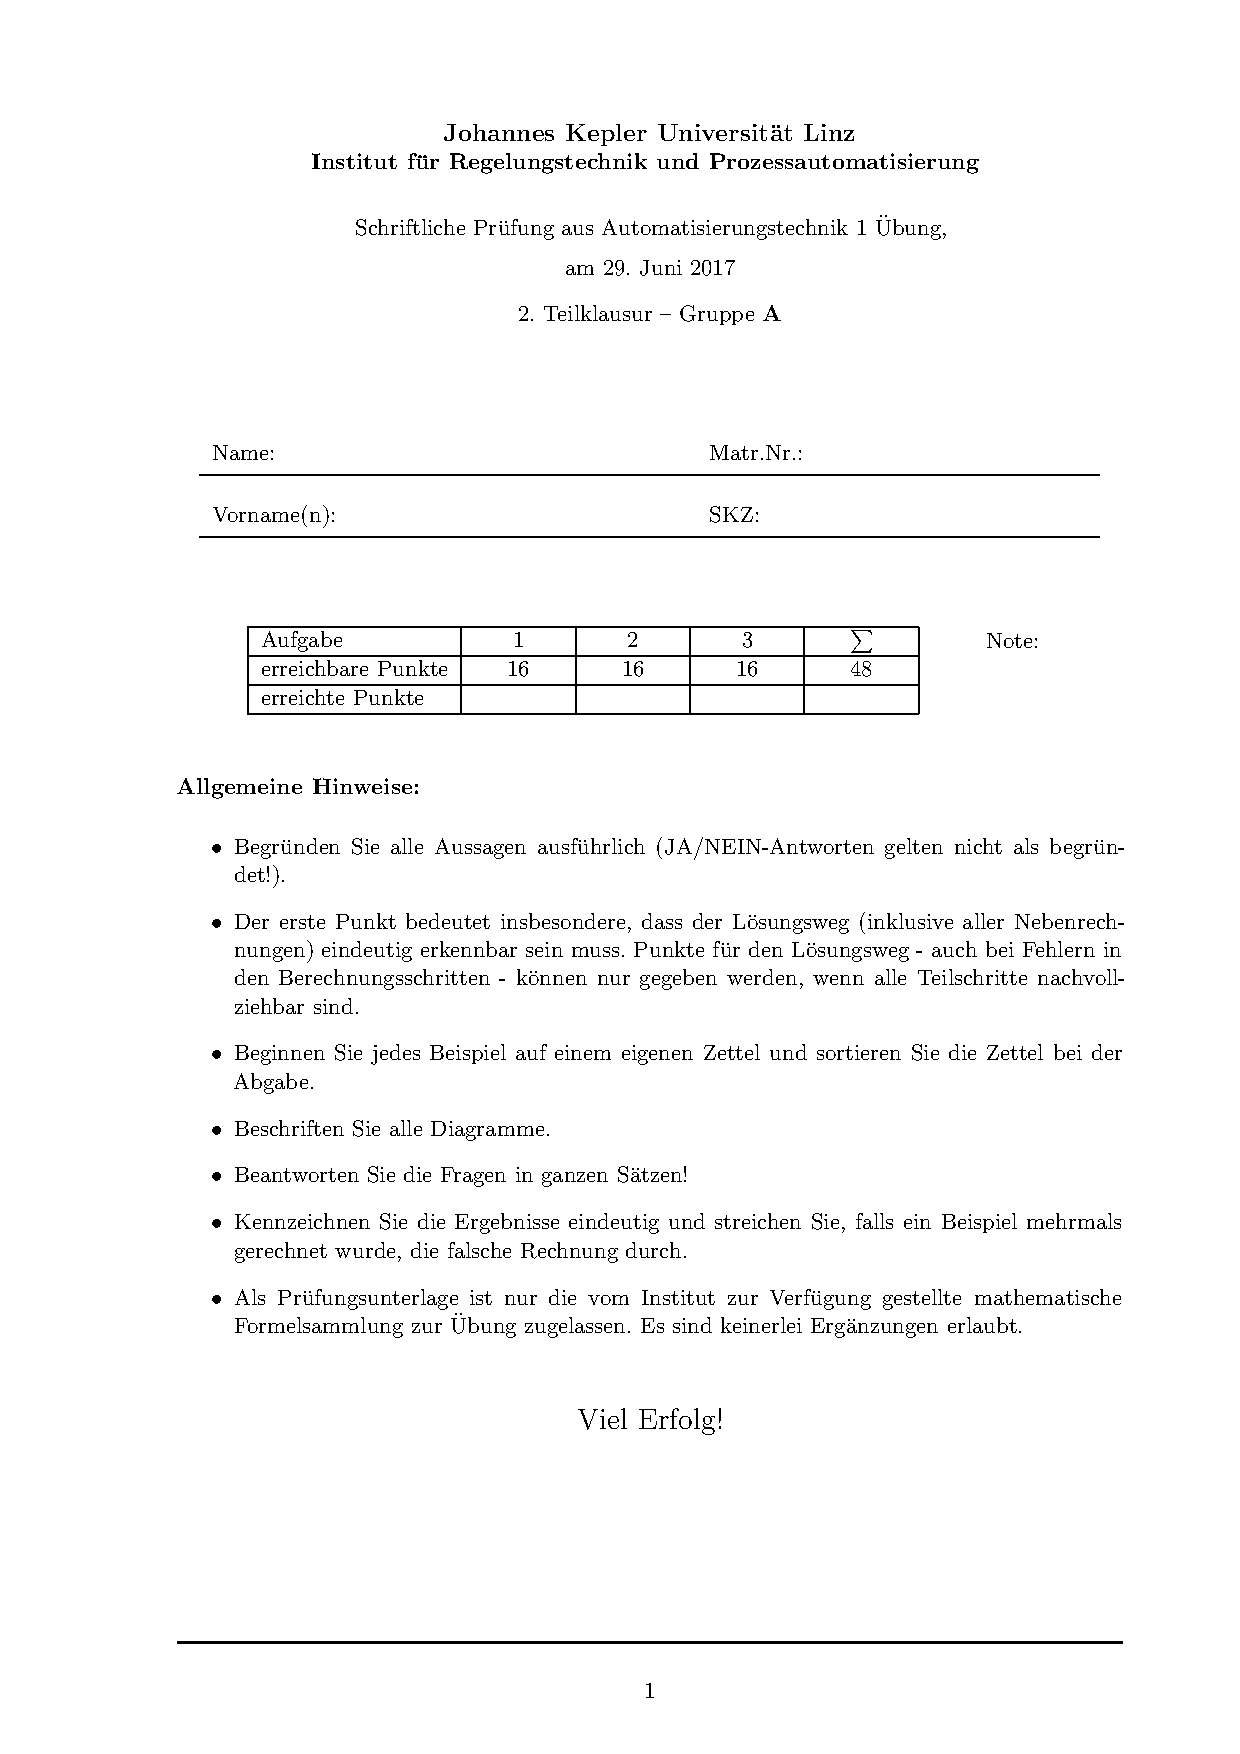
\includepdf[pages=-]{KlausurA_2017_06_29_nachtrKorrigiert}

\begin{task}[Erreichbarkeit und Zustandsregler]
Betrachten Sie das LTI-System

$$ 
\begin{aligned} \dot{\mathbf{x}} &=\mathbf{A x}+\mathbf{b} u, \quad \mathbf{x}(0)=\mathbf{x}_{0} \\ y &=\mathbf{c}^{T} \mathbf{x} \end{aligned}
 $$
mit den Matrizen
 $$ 
\mathbf{A}=\left[\begin{array}{cc}{1} & {2} \\ {-1} & {0}\end{array}\right], \quad \mathbf{b}=\left[\begin{array}{l}{1} \\ {0}\end{array}\right], \quad \mathbf{c}^{\top}=\left[\begin{array}{ll}{2} & {0}\end{array}\right]
 $$
 \begin{enumerate}[i]
  \item Zeigen Sie, dass das System vollständig erreichbar ist
\begin{solution}
Es ist zu prüfen ob die Matrix $\mathbf{M}_R = \left[\mathbf{b}, \mathbf{Ab} \right]$ vollen Rang besitzt.

\[ \text{rank}\left(\mathbf{M}_R\right) = \text{rank}\left(\begin{pmatrix} 1 & 1 \\ 0 & -1 \end{pmatrix}\right)=2=n \rightarrow \text{vollständig erreichbar}\]
\end{solution}
  \item Berechnen Sie mit Hilfe der Formel von Ackermann einen Zustandsregler so, dass
die Eigenwerte des geschlossenen Kreises bei $\{-2,-2\}$ liegen.
\begin{solution}
Mit Hilfe der Formel von Ackermann kann der Rückführvektor $\mathbf{k}^{T}$ direkt aus
\[ 
\mathbf{k}^{T}=-\alpha_{0} \mathbf{t}_{1}^{T}-\alpha_{1} \mathbf{t}_{1}^{T} \mathbf{A}-\cdots-\alpha_{n-1} \mathbf{t}_{1}^{T} \mathbf{A}^{n-1}-\mathbf{t}_{1}^{T} \mathbf{A}^{n}
 \]
 berechnet werden. Für $\mathbf{t}_{1}^{T}$ gilt $\mathbf{e}_{n}^{T}=\mathbf{t}_{1}^{T} \mathbf{M}_{R}$.
 
 $\mathbf{t}_{1}^{T}$ ist also $\begin{pmatrix} 0 & -1\end{pmatrix}$.\\ Die Koeffizienten $\alpha_i$ sind die Koeffizienten des charakteristischen Polynoms:
 \[ 
p(s)=\alpha_{0}+\alpha_{1} s+\cdots+\alpha_{n-1} s^{n-1}+s^{n}
 \]
 Durch die Polvorgabe ergibt sich folgendes charakteristische Polynom:
  \[ 
p(s)=(\lambda+2)(\lambda+2)= 4+4\lambda+\lambda^2 \rightarrow \alpha_0 = 4, \alpha_1 = 4
 \]
 Damit kann $\mathbf{k}^{T}$ berechnet werden:
 \[ 
\mathbf{k}^{T}=-\alpha_{0} \mathbf{t}_{1}^{T}-\alpha_{1} \mathbf{t}_{1}^{T} \mathbf{A}-\mathbf{t}_{1}^{T} \mathbf{A}^{2}
 \]
 \[
 \mathbf{k}^{T}=-4 \begin{pmatrix} 0 & -1\end{pmatrix}-4 \begin{pmatrix} 0 & -1\end{pmatrix} \left[\begin{array}{cc}{1} & {2} \\ {-1} & {0}\end{array}\right]-\begin{pmatrix} 0 & -1\end{pmatrix} \left[\begin{array}{cc}{1} & {2} \\ {-1} & {0}\end{array}\right]^{2}
 \]
  \[
 \mathbf{k}^{T}=-4 \begin{pmatrix} 0 & -1\end{pmatrix}-4 \begin{pmatrix} 1 & 0\end{pmatrix} -\begin{pmatrix} 1 & 2\end{pmatrix} = \begin{pmatrix} -5 & 2\end{pmatrix}
 \]
\end{solution}
  \item Geben Sie den Grenzwert $\lim _{t \rightarrow \infty} x_{1}(t)$ für den geschlossenen Kreis mit
$\mathrm{x}_{0}=[2,-1]^{\top}$ an.
\begin{solution}
Im geschlossenen Kreis handelt es sich um ein stabiles System mit negativen Eigenwerten. Das System tendiert nach unendlich langer Zeit zum Zustand $\mathbf{x} = \mathbf{0}$.\\
$\lim _{t \rightarrow \infty} x_{1}(t) = 0$
\end{solution}
\end{enumerate}
\end{task}

\begin{task}
Gegeben ist das System der Form
\[ 
\begin{aligned} \dot{\mathbf{x}} &=\left[\begin{array}{cc}{\alpha_{1}} & {0} \\ {0} & {\alpha_{2}}\end{array}\right] \mathbf{x}+\left[\begin{array}{c}{\beta_{1}} \\ {\beta_{2}}\end{array}\right] u \\ y &=\left[\begin{array}{ll}{1} & {2}\end{array}\right] \mathbf{x} \end{aligned}
 \]
 \begin{enumerate}[i]
     \item Bestimmen Sie den Wertebereich für $\alpha_{1}, \alpha_{2}, \beta_{1}, \beta_{2}$ so, dass die Dimension des erreichbaren Unterraums dim $(\mathcal{R})=1$ gilt.
     \begin{solution}
     \[ \mathcal{R} = \text{span}\left(\mathbf{b},\mathbf{Ab}\right)\]
     Damit dieser Vektorraum eindimensional wird, muss $\mathbf{b}$ linear abhängig von $\mathbf{Ab}$ sein, $\mathbf{b}$ also ein rechtseigenvektor von $\mathbf{A}$ sein.
     \[\text{Dim}\left(\mathbf{M}_R\right)=
     \text{Dim}\left(
     \begin{pmatrix}
     \beta_1 & \alpha_1 \beta_1 \\
     \beta_2 & \alpha_2 \beta_2
     \end{pmatrix}
     \right)
     \stackrel{!}{=} 1
     \]
     Um diese Bedingung zu erfüllen darf weder $\beta_1$ noch $\beta_2$ 0 sein, dies führte zu einer Nullmatrix mit Rang 0 führen.
     \[\rightarrow \beta_1 \neq 0 \quad \beta_2 \neq 0\]
     \end{solution}
     \item Es gelte nun $\operatorname{dim}(\mathcal{R})=1, \alpha_{2}=2$ und $\beta_{1}=\beta_{2}=1$
     \begin{enumerate}[A]
         \item Bestimmen sie $\alpha_{1}$ und transformieren Sie das System in ein erreichbares Teilsystem und ein Restsystem. Geben Sie die Transformationsvorschrift sowie
das System in transformierten Koordinaten z explizit an.
\begin{solution}
\[\text{Dim}\left(\mathbf{M}_R\right)=
     \text{Dim}\left(
     \begin{pmatrix}
     1 & \alpha_1 \\
     1 & 2
     \end{pmatrix}
     \right)
     \stackrel{!}{=} 1 \rightarrow \alpha_1 = 2
     \]
     
     Basis für den erreichbaren Zustandsraum: $\begin{pmatrix}1&1\end{pmatrix}^T$, Komplementärvektor um den ganzen $\mathbb{R}^2$ aufzuspannen: $\begin{pmatrix}0&1\end{pmatrix}^T$
     
     Transformationsmarix: $ V = \begin{pmatrix} 1 & 0 \\ 1 & 1 \end{pmatrix},V^{-1} = \begin{pmatrix} 1 & 0 \\ -1 & 1 \end{pmatrix}$
     
     \[\mathbf{x} = \mathbf{V}\mathbf{z}, \ \mathbf{V}^{-1}\mathbf{x} = \mathbf{z}\]
     \[\dot{\mathbf{z}}=\mathbf{V}^{-1}\dot{\mathbf{x}} = \mathbf{V}\mathbf{A}^{-1}\mathbf{x} + \mathbf{V}^{-1}\mathbf{b}u = \underbrace{\mathbf{V}^{-1}\mathbf{A}\mathbf{V}}_{\overline{\mathbf{A}}}\mathbf{z} + \underbrace{\mathbf{V}^{-1}\mathbf{b}}_{\overline{\mathbf{b}}}u\]
     \[y = \mathbf{c}^T \mathbf{x} = \underbrace{\mathbf{c}^T \mathbf{V}}_{\overline{\mathbf{c}^T}}\mathbf{z}\]
     
     Das transformierte System lautet explizit:
     \[ \dot{\mathbf{z}} =  \overline{\mathbf{A}} z + \overline{\mathbf{b}}u = \begin{pmatrix}2&0\\0&2\end{pmatrix}z+\begin{pmatrix}1\\0\end{pmatrix}u\]
     \[ y = \overlien{\mathbf{c}^T}\mathbf{z} = \begin{pmatrix}3&2\end{pmatrix}\mathbf{z} \]
     Das System ist nicht vollständig erreichbar. Der zweite Eintrag des Zustandsvektors wird durch ein autonomes Differentialgleichungssystem beschrieben. Weder der erste Zustand noch der Eingang $u$ haben eine Auswirkung auf dieses Teilsystem.
\end{solution}
        \item Ist das System stabilisierbar? \emph{Begründung!}
        \begin{solution}
        Das System ist \emph{nicht} stabilisierbar. Die Systemmatrix ($\mathbf{A}_{22})$ des nicht-erreichbaren Teilsystem müsste Hurwitz sein, hat hier jedoch den Eigenwert 2.
        \end{solution}
     \end{enumerate}
 \end{enumerate}
\end{task}
\begin{task}{Beobachtbarkeit und Beobachterentwurf}
Für das LTI-System
\[\begin{aligned} \dot{\mathbf{x}} &=\left[\begin{array}{cc}{2} & {0} \\ {-2} & {-1}\end{array}\right] \mathbf{x}+\left[\begin{array}{c}{1} \\ {0}\end{array}\right] u \\ y &=\left[\begin{array}{cc}{2} & {0}\end{array}\right] \mathbf{x}-3 u \end{aligned}\]
soll ein vollständiger Beobachter entworfen werden. Bearbeiten Sie dazu folgende Unterpunkte
\begin{enumerate}[i]
    \item Können die Eigenwerte des Fehlersystems durch geeignete Wahl von $\hat{\mathrm{k}}$ beliebig
platziert werden? Falls NEIN, geben Sie die nicht beeinflussbaren Eigenwerte des
Fehlersystems an. \emph{Begründung!}
\item Geben Sie das Fehlersystem für die Wahl $\hat{\mathbf{k}}=\left[\begin{array}{cc}{-2} & {2}\end{array}\right]^{\top}$ an.
\item Der Beobachter wird als dynamisches System der Form
\[\begin{aligned} \dot{\mathbf{z}} &=\mathbf{A}_{B} \mathbf{z}+\mathbf{B}_{B} \mathbf{w} \\ \hat{\mathbf{x}} &=\mathbf{C}_{B} \mathbf{z}+\mathbf{D}_{B} \mathbf{w} \end{aligned}\]
mit dem Zustand z und dem Eingang w implementiert. Geben Sie w sowie die
Matrizen $\mathbf{A}_{B}, \mathbf{B}_{B}, \mathbf{C}_{B}$ und $\mathbf{D}_{B}$ unter Verwendung von $\hat{\mathbf{k}}$ aus Punkt (ii) explizit
an.

\end{enumerate}

\end{task}

\end{document}
